%%%%%%%%%%%%%%%%%%%%%%%%%%%%%%%%%%%%%%%%%
% Beamer Presentation
% LaTeX Template
% Version 1.0 (10/11/12)
%
% This template has been downloaded from:
% http://www.LaTeXTemplates.com
%
% License:
% CC BY-NC-SA 3.0 (http://creativecommons.org/licenses/by-nc-sa/3.0/)
%
%%%%%%%%%%%%%%%%%%%%%%%%%%%%%%%%%%%%%%%%%

%----------------------------------------------------------------------------------------
%	PACKAGES AND THEMES
%----------------------------------------------------------------------------------------

\documentclass[c]{beamer}
%\documentclass[notes]{beamer}
\setbeamertemplate{note page}[show only notes]
\input{../OR_common.tex}
%%%%%%%%%%%%%%%%%%%%%%%%%%%%%%%%%%%%%%%%%%%%%%%%%%%%%%%%%%%%%%%%%%%%%%%%%%%%%
%%%%%%%%%%%%%%%%%%%%%%%%%%%%%%%%%%%%%%%%%%%%%%%%%%%%%%%%%%%%%%%%%%%%%%%%%%%%%
%%%%%%%%%%%%%%%%%%%%%%%%%%%%%%%%%%%%%%%%%%%%%%%%%%%%%%%%%%%%%%%%%%%%%%%%%%%%%

\title[Introduction]{Unit 2. Linear programming. Duality}

\author{Jordi Villà i Freixa}
\institute[FCTE]{
Universitat de Vic - Universitat Central de Catalunya \\
Study Abroad. Operations Research\\
\medskip
\textit{jordi.villa@uvic.cat}
}
\date{25/04-2/05, 2023}
\logo{
\includegraphics[width=.1\textwidth]{FCTE}}
\begin{document}

\begin{frame}
\titlepage
\end{frame}


\begin{frame}
    \frametitle{Preliminary}
    This course is strongly based on the monography on Operations Research by Carter, Price and Rabadi \cite{carter}, and in material obtained from different sources (quoted when needed through the slides).
\end{frame}

%%%%%%%%%%%%%%%%%%%%%%%%%%%%%%%%%%%%%%%%%%%%%%%%%%%%%%%%%%%%%%%%%%%%%%%%%%%%%
%%%%%%%%%%%%%%%%%%%%%%%%%%%%%%%%%%%%%%%%%%%%%%%%%%%%%%%%%%%%%%%%%%%%%%%%%%%%%
%%%%%%%%%%%%%%%%%%%%%%%%%%%%%%%%%%%%%%%%%%%%%%%%%%%%%%%%%%%%%%%%%%%%%%%%%%%%%

\begin{frame}
\frametitle{Learning outcomes}
\begin{itemize}
  \item Understanding Dual and Primal problems in LP
  \item Economic interpretation
  \item Conditions of optimality
  \item Resolution of the dual by the primal and penalty method
\end{itemize}
\end{frame}

\section{Duality}
\note{\url{https://www.youtube.com/watch?v=yU8updOR87c}}
\begin{frame}{A first example}

  \begin{equation*}
    \begin{aligned}
      \text{maximize  } \quad & 4x_1 + x_2 +5x_3 +3x_4 \\
      \text{subject to }\quad &
      \left\{
      \begin{array}{rcl}
        x_1 - x_2 -x_3 +3x_4 &\leq &1 \\
        5x_1 + x_2 +3x_3 +8x_4 &\leq &55 \\
        -x_1 + x_2 +3x_3 -5x_4 &\leq &3 \\
        x_1,x_2,x_3 &\geq& 0
      \end{array}
      \right.
    \end{aligned}
  \end{equation*}

\end{frame}
  \begin{frame}{A first example}
note that

\begin{eqnarray*}
  y_1(x_1 - x_2 -x_3 +3x_4)+\\y_2(5x_1 + x_2 +3x_3 +8x_4)+\\y_3(-x_1 + x_2 +3x_3 -5x_4) \\ \leq \\y_1+55y_2+3y_3
\end{eqnarray*}

\end{frame}
\begin{frame}{Primal and Dual}

We see that maximizing the {\bf Primal objective function} $4x_1 + x_2 +5x_3 +3x_4$ is
  equivalent to minimize the {\bf Dual objective function} $y_1+55y_2+3y_3$:

    \begin{equation*}
    \begin{aligned}
      \text{minimize } \quad & y_1+55y_2+3y_3 \\
      \text{subject to }\quad &
      \left\{
      \begin{array}{rcl}
        y_1 - 5y_2 -y_3 &\geq &4 \\
        -y_1 +y_2 +2y_3 &\geq &1 \\
        -y_1 +3y_2 +3y_3 &\geq &5 \\
        3y_1 +8y_2 -5y_3 &\geq &3 \\
        y_1,y_2,y_3,y_4 &\geq& 0
      \end{array}
      \right.
    \end{aligned}
  \end{equation*}

  \end{frame}


\begin{frame}{Generalization}
In general, if we can write the LP problem in its {\bf normal formulation}:
\[
\begin{rcases}
\text{min }\quad\uvec{c}^t \uvec{x}\\
\text{subject to }\quad A\uvec{x}\geq \uvec{b}, \forall x_i\geq0
\end{rcases} \text{PRIMAL}
\]

\[
\begin{rcases}
\text{max }\quad\uvec{b}^t \uvec{y}\\
\text{subject to }\quad A^t\uvec{y}\leq \uvec{c}, \forall y_i\geq0
\end{rcases} \text{DUAL}
\]
The dual problem is a transposition of the primal problem.
\end{frame}

\begin{frame}{}
\begin{Exercise}
  Find the dual problem of
  \begin{equation*}
  \begin{aligned}
    \text{maximize } \quad & 3x_1 +2x_2 \\
    \text{subject to }\quad &
    \left\{
    \begin{array}{rcl}
      2x_1+x_2 &\leq &4 \\
      2x_1+3x_2 &\leq &6 \\
      x_1,x_2 &\geq& 0
    \end{array}
    \right.
  \end{aligned}
\end{equation*}
Solve it graphically and using Simplex.
\end{Exercise}
\end{frame}
\note{\begin{center}
  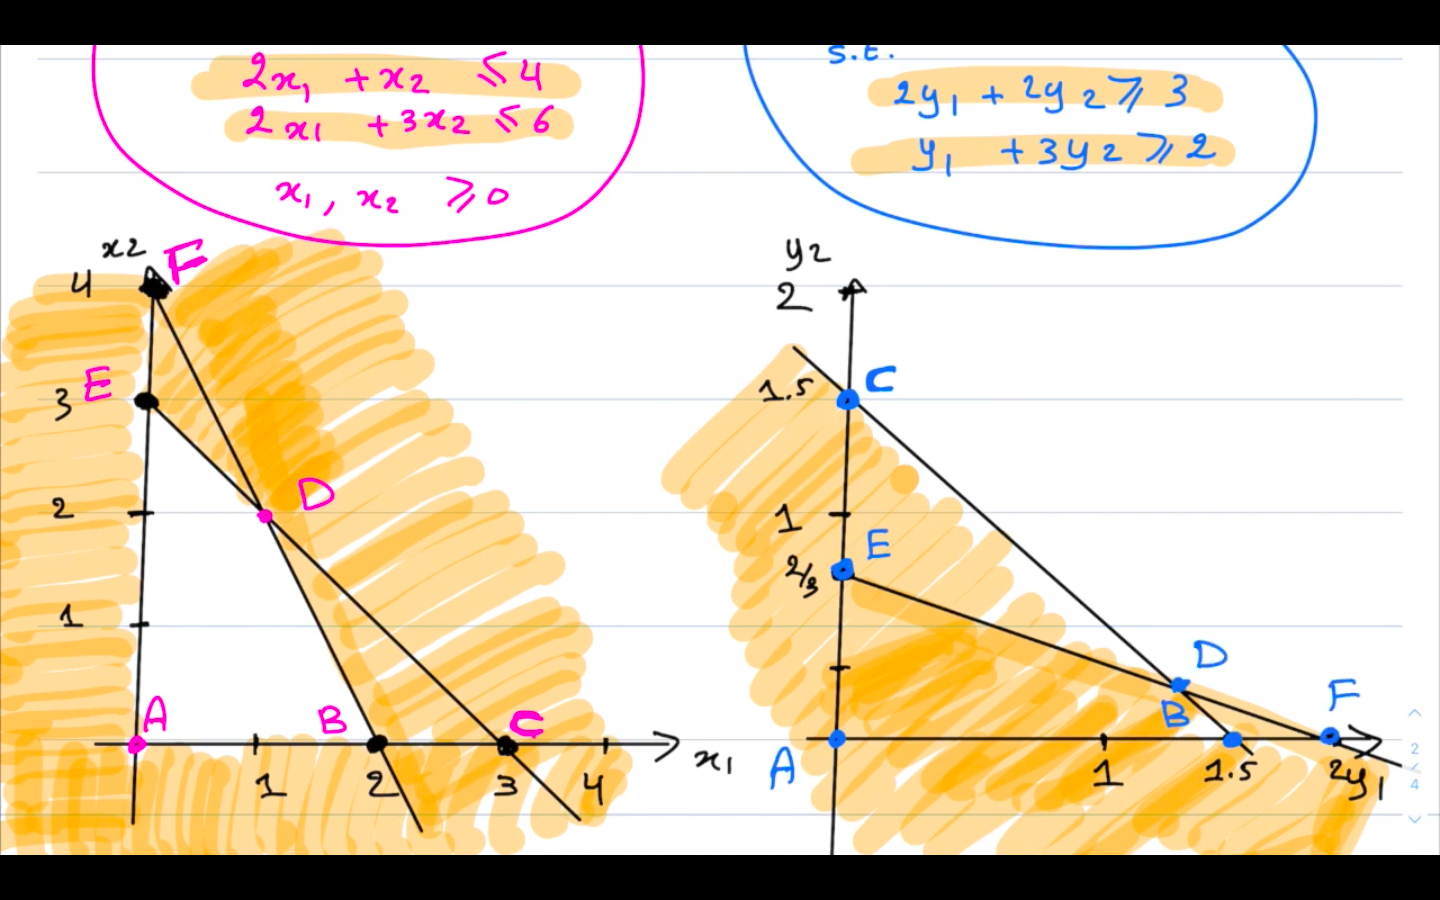
\includegraphics[width=0.8\linewidth]{answer1.png}
  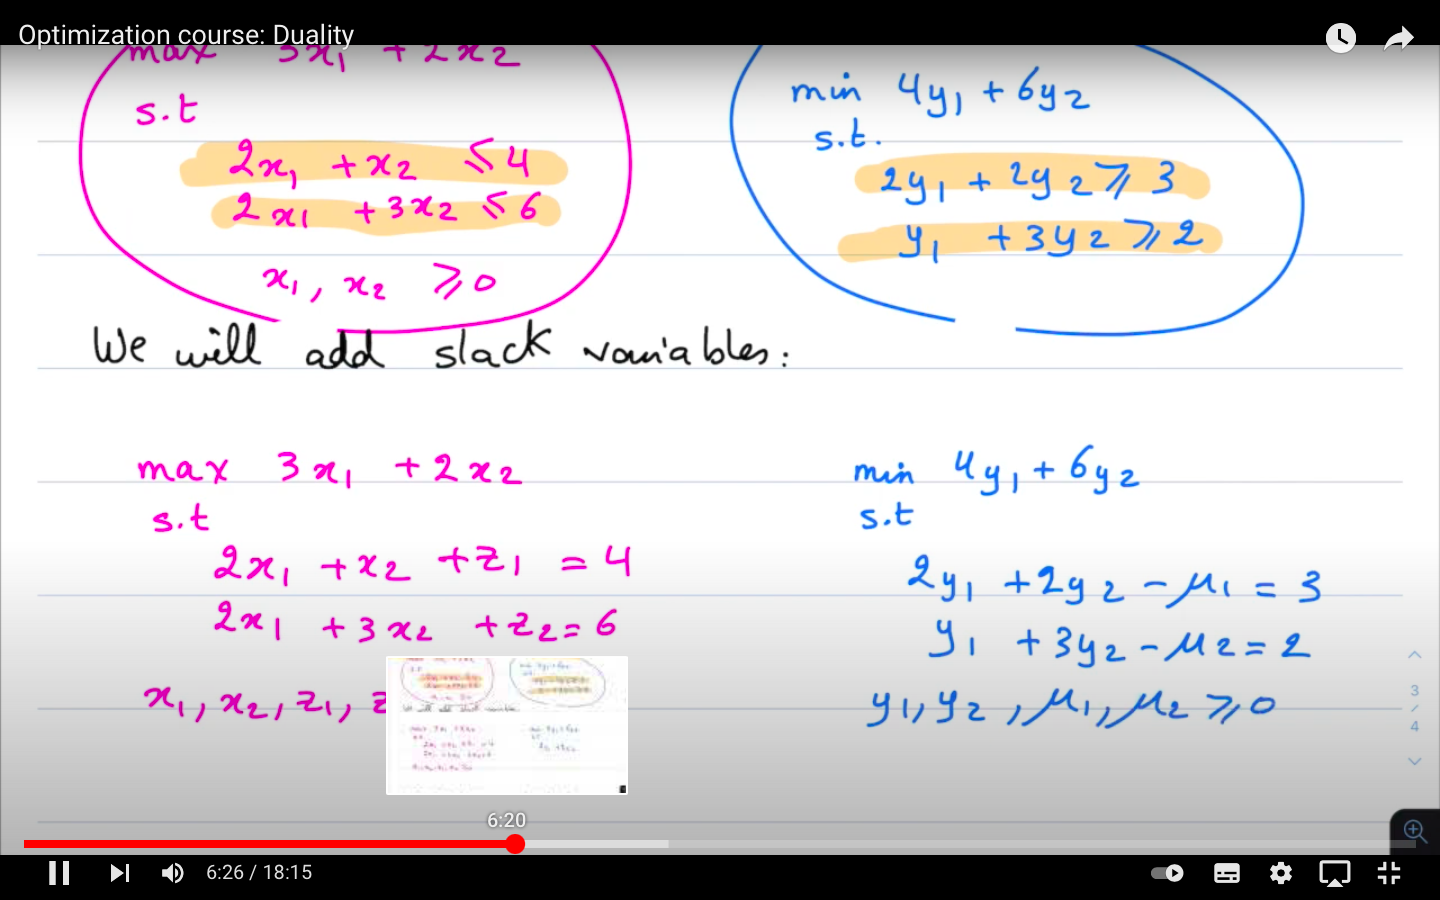
\includegraphics[width=0.8\linewidth]{answer3.png}
  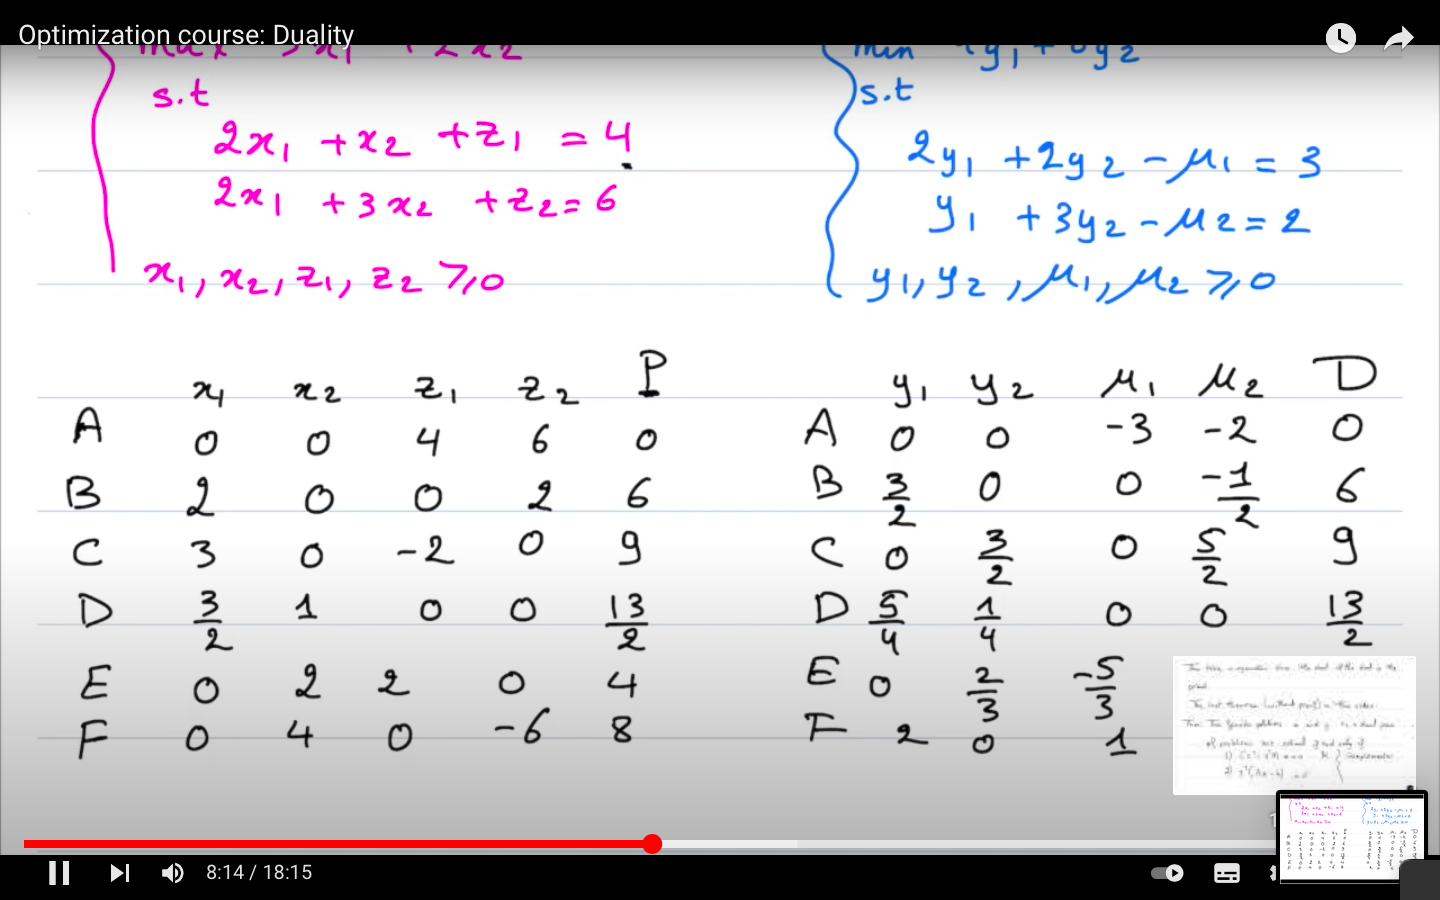
\includegraphics[width=0.8\linewidth]{answer2.png}
  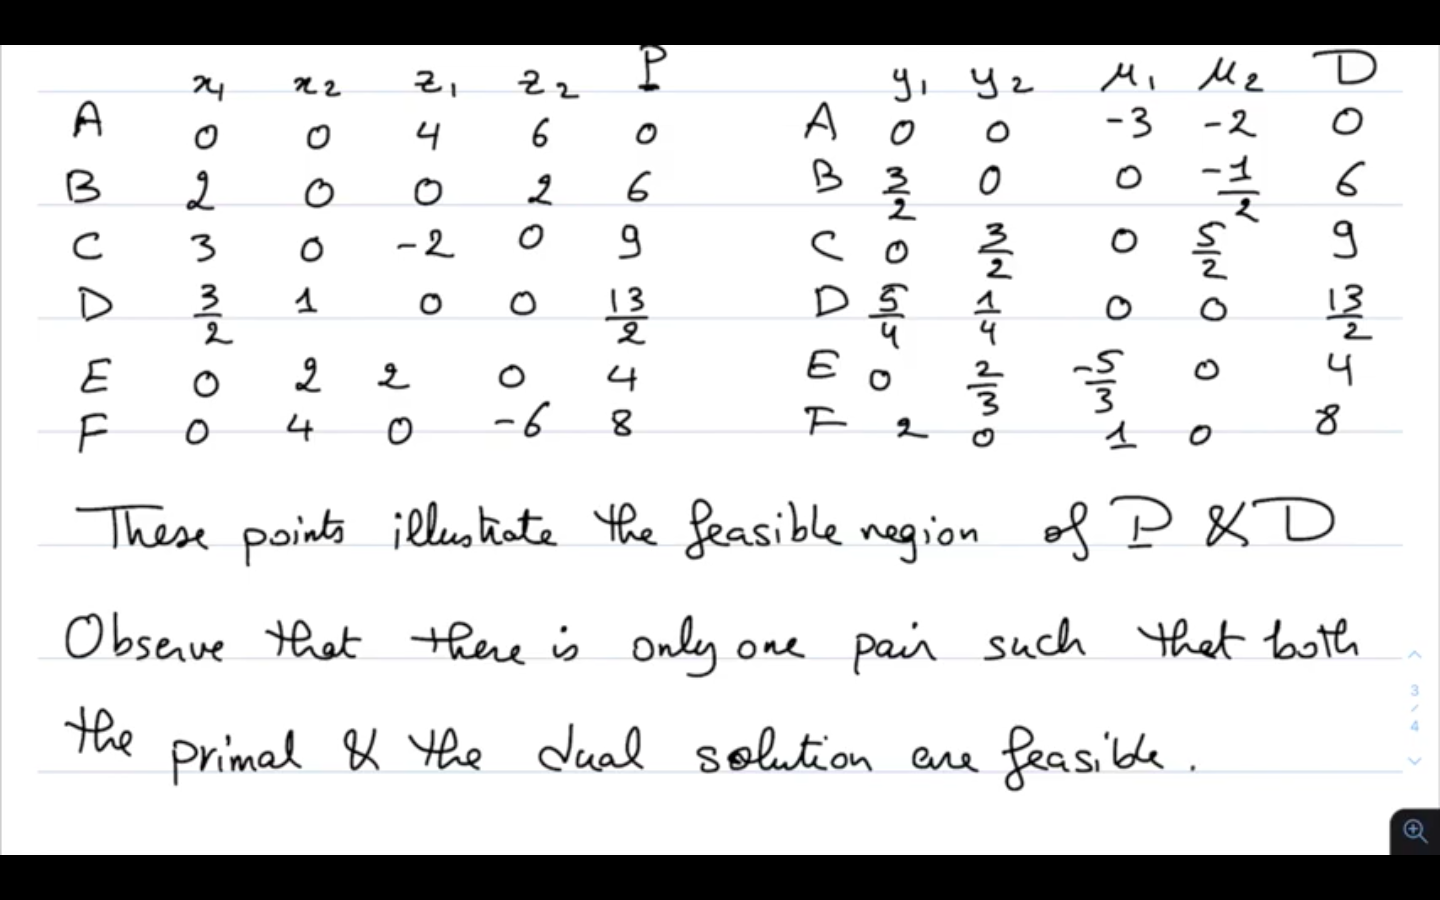
\includegraphics[width=0.8\linewidth]{answer4.png}
\end{center}
}

\begin{frame}{}
\begin{Exercise}
  Find the dual problem of
  \begin{equation*}
  \begin{aligned}
    \text{minimize } \quad & 4x_1 +4x_2+x_3 \\
    \text{subject to }\quad &
    \left\{
    \begin{array}{rcl}
      x_1+x_2+x_3 &\leq &2 \\
      2x_1+x_2 &= &3 \\
      2x_1+x_2+3x_3 &\geq &3 \\
      x_1,x_2,x_3 &\geq& 0
    \end{array}
    \right.
  \end{aligned}
\end{equation*}
Trick: normalize the problem first: eg $2x_1+x_2=3 \rightarrow \begin{cases}2x_1+x_2 \geq 3\\2x_1+x_2\leq 3\end{cases}$.
\end{Exercise}
\end{frame}
\note{
\url{https://www.youtube.com/watch?v=wVnr1HhUCT0}
}

\section{Some theory}

\begin{frame}{Dual of the dual}
\begin{theorem}
  In the case of linear programming, the dual of the dual is the primal.
\end{theorem}
\begin{proof}
 \[
\begin{rcases}
\text{max }\quad\uvec{b}^t \uvec{y}\\
\text{subject to }\quad A^t\uvec{y}\leq \uvec{c}, \forall y_i\geq0
\end{rcases} \text{DUAL}
\]
is equivalent to
\[
\begin{rcases}
\text{min }\quad-\uvec{b}^t \uvec{y}\\
\text{subject to }\quad -A^t\uvec{y}\geq -\uvec{c}, \forall y_i\geq0
\end{rcases} \text{DUAL}
\]
where, by taking again the Dual, leads to the original Primal.
\end{proof}
\end{frame}

\begin{frame}[allowframebreaks]{Meaning of Duality}
  Let us retake the example we saw in the last session:

  \begin{equation*}
    \begin{aligned}
      \text{maximize } \quad & z = 8x_1+5x_2 \\
      \text{subject to }\quad &
      \begin{array}{rcl}
        x_1 &\leq &150 \\
        x_2 &\leq &250 \\
        2x_1+x_2 &\leq &500 \\
        x_1,x_2 &\geq& 0
      \end{array}
    \end{aligned}
  \end{equation*}

  We found out that, from the initial tableau:

\begin{equation*}
\begin{array}{cc}
&\\
&z \\
\rightarrow &s \\
&t \\
&u\\
\mathrm{basic}
\end{array}
%
\begin{array}{c|ccccc|c}
  z & x_1 & x_2 & s & t & u & b \\ \hline
  1 & -8 & -5 & 0 & 0 & 0 & 0 \\ \hline
  0 & 1 & 0 & 1 & 0 & 0 & 150  \\
  0 & 0 & 1 & 0 & 1 & 0 & 250 \\
  0 & 2 & 1 & 0 & 0 & 1 & 500 \\
    & \uparrow & & & & &
\end{array}
%\end{matrix}
\end{equation*}

and after applying the different steps of the Simplex method we ended up with the final tableau:

  \begin{equation*}
  \begin{array}{cc}
  &\\
  R_1+5R_4&z \\
  &x_1 \\
  \rightarrow R_3-R_4&s \\
  &x_2\\
  &\mathrm{basic} \\
  \end{array}
  \begin{array}{c|ccccc|c}
    z & x_1 & x_2 & s & t & u & b \\ \hline
    1 & 0 & 0 & 0 & 1 & 4 & 2250 \\ \hline
    0 & 1 & 0 & 0 & -1/2 & 1/2 & 125  \\
    0 & 0 & 0 & 1 & 1/2 & -1/2 & 25 \\
    0 & 1 & 0 & 1 & 0 & 0 & 250 \\
      &  & & \uparrow& & &
  \end{array}
  \end{equation*}

Now, if we multiply the original availability of each resource (shown in the original tableau) by its marginal worth (taken from the final tableau) and get the sum, we obtain the optimal objective function value:

\[
z* = 2250 = 0(150)+1(250)+4(500)
\]

\end{frame}

\begin{frame}{Duality properties}


\begin{theorem}[Weak Duality]
  In a max LP, the value of primal objective function for any feasible solution is bounded from above by any feasible solution to its dual:
  \[\text{max } \qquad \bar{z} \leq \bar{w} \]
\end{theorem}
The statement is analogous to a minimization problem.
\begin{theorem}[Unboundness property]
  If primal (dual) problem has an unbounded solution, then the dual (primal) is unfeasible.
  \[\text{max } \qquad \bar{z} \leq \infty \]
\end{theorem}
\end{frame}

\begin{frame}{Duality properties}


\begin{theorem}[Strong Duality]
  If the primal problem has an optimal solution,
  \[
  x^* = (x_1^*, \ldots, x_n^*)
  \]
  the the dual also has an optimal solution,
  \[
  y^* = (y_1^*, \ldots, y_m^*)
  \]
and
\[
z^* := \sum_j c_j x_j^* = \sum_i b_i y_i^* := w^*
\]

\end{theorem}
Thus: if feasible objective function values are found for a primal and dual pair of problems, and if these values are equal to each other, then both of the solutions are optimal solutions.

The Shadow prices that appear at the top of the optimal tableau of the primal problem are precisely the optimal values of the dual variables!
\end{frame}

\begin{frame}{Cases with no optimal solutions for primal and dual}
  Exactly one of the following mutually exclusive cases always occurs:
  \begin{itemize}
    \item Both primal and dual problems are feasible, and both have optimal (and equal) solutions.
    \item Both primal and dual problems are infeasible (have no feasible solution).
    \item The primal problem is feasible but unbounded, and the dual problem is infeasible.
    \item The dual problem is feasible but unbounded, and the primal problem is infeasible.
  \end{itemize}
\end{frame}

\begin{frame}{Complementary slackness}
  Because each decision variable in a primal problem is associated with a constraint in the dual problem, each such variable is also associated with a slack or surplus variable in the dual.

  In any solution, if the primal variable is basic (with value $\geq0$, hence having slack), then the associated dual variable is non-basic ($=0$, hence having no slack), and viceversa.

  \begin{theorem}
    If in an optimal solution to a LP problem and inequality constraint is not binding, then the dual variable corresponding to that constraint has a value of zero in any optimal solution to the dual problem. In other words: suppose $x_0$ and $y_0$ are feasible solutions of (max) and (min) representations. Then, $x_0,y_0$ are optimal solutions if and only if
    \begin{eqnarray*}
      (b-Ax_0)\cdot y_0 =0\\
      (A^ty_0-c) \cdot x_0 =0
    \end{eqnarray*}
  \end{theorem}
\end{frame}
\note{Veure exemple pràctic a \url{https://youtu.be/o1pznRt_-y0?t=1603}}



\section{References}
\begin{frame}{References}
    \footnotesize
    \begin{thebibliography}{99}
    \setbeamertemplate{bibliography item}[text]
      \begin{columns}[t]
        \begin{column}{.45\textwidth}
            \bibitem{carter} Michael W. Carter, Camille C. Price, and Ghaith Rabadi. Operations Research, 2nd Edition. CRC Press.
            \bibitem{harel} David Harel, with Yishai Feldman. Algorithmics: the spirit of computing, 3rd Edition. Addison-Wesley.
            \bibitem{rardin} Ronald L. Rardin. Optimization in Operations Research, 2nd Edition. Pearson.
            \bibitem{hefferon} J. Hefferon. \href{http://joshua.smcvt.edu/linearalgebra}{Linear algebra (4th Ed)}.
        \end{column}
        \begin{column}{.45\textwidth}
            \bibitem{riley} K.F. Riley, M.P. Hobson, S.J. Bence. Mathematical Methods for Physics and Engineering (2nd Ed). McGraw Hill.
            \bibitem{nocedal} J. Nocedal, S. J. Wright. Numerical Optimization (2nd Ed). Springer.
            \bibitem{beers} Kenneth J. Beers. Numerical methods for chemical engineering: applications in Matlab. Cambridge University Press.
            \bibitem{barber} D. Barber. Bayesian reasoning and machine learning. Cambridge University Press.
        \end{column}
      \end{columns}
    \end{thebibliography}
\end{frame}
%----------------------------------------------------------------------------------------

\end{document}
